\section{Self-gravitating matter}\label{sec:selfgravity}

Coupled Einstein-Vlasov dynamics begins once macroparticles carry finite rest mass $m_p$ and feed their deposited sources $(E, S_i, S_{ij})$ back into the spacetime evolution. Collective gravitational wells then form, oscillate, disperse, or collapse into black holes from the matter distribution itself, closing the particle-mesh cycle of Sec.~\ref{sec:method}. Whereas Ref.~\cite{Wu:2026nrpic} evolves its main self-gravitating benchmarks with about $10^6$ to $5 \times 10^6$ macroparticles on large machines, every run here uses at most ten thousand ($N \le 10^4$) on one graphics card. Quantities independent of $N$, such as continuum equilibrium sequences and analytic collapse bounds, test the coupled solver at full precision. Phenomena sensitive to discrete sampling---initial lattices, multi-pass filtering, refinement under diffuse matter, and cluster holding---isolate what changes at $N \le 10^4$, with scenario parameters listed in the appendix.

\subsection{Dust collapse}\label{sec:dust}

Spherical collapse of cold, pressureless matter from rest tests the coupled solver from smooth initial curvature through black hole formation against an exact solution \cite{Oppenheimer:1939ue}. A homogeneous dust ball of initial areal radius $R_0 = 5\,M$, ADM mass $M$, and uniform density $E_0 = \rho_0 = 3M/(4\pi R_0^3)$ starts at rest on a conformally flat slice \cite{Petrich:1985jko,Staley:2011ss,Wu:2026nrpic}. At $t = 0$, momenta $u_{i,p}$, extrinsic curvature $K_{ij}$, and shift $\beta^i$ vanish, $\alpha = 1$, and interior and exterior $\psi$ join smoothly at isotropic radius $\rbar_0$. Nearly $10^4$ macroparticles occupy a cubic lattice of spacing $h$ inside $\rbar_0$ and evolve with dynamic refinement, one plain binomial filter pass, and lapse excision. Along free-falling worldlines parameterized by $\varphi \in [0, \pi)$, shell areal radius $R$, central proper time $\tau_c$, and interior density $E$ follow the cycloid \cite{Oppenheimer:1939ue},
\begin{align}\label{eq:cycloid}
R(\varphi) &= \frac{R_0}{2}(1 + \cos\varphi), \qquad
\tau_c(\varphi) = \sqrt{\frac{R_0^3}{8M}}\,(\varphi + \sin\varphi), \nonumber\\
E(\varphi) &= E_0\!\left(\frac{R_0}{R(\varphi)}\right)^3.
\end{align}
Because $1+\log$ slicing ties $\partial_t\alpha$ to local volume contraction, $\alpha_c$ tracks central compression directly. From unit initial lapse without shift advection, local integration inside the homogeneous core gives an analytic lower bound on $\alpha_c$, the lapse bound \cite{Staley:2011ss},
\begin{equation}\label{eq:lapse_bound}
\alpha_{\rm bound}(\tau_c) = 1 + 6\ln\!\left(\frac{R(\tau_c)}{R_0}\right).
\end{equation}
The surface density jump launches an inward gauge wave in the slicing coordinate $\alpha$. Until that gauge wave reaches the origin, causal isolation keeps $\alpha_c(\tau_c)$ on the lapse bound while the dust falls freely.

Central infall and black hole formation are expected to match continuum Oppenheimer--Snyder collapse despite the discrete particle representation. In the simulation (Fig.~\ref{fig:dust}, top left), $\alpha_c(\tau_c)$ tracks the lapse bound closely during causal isolation and departs smoothly once the surface gauge wave arrives, matching Ref.~\cite{Wu:2026nrpic} and continuum runs \cite{Staley:2011ss}. Until the center refines to $\Delta x = h/4$, the central density $E_c(\tau_c)$ likewise follows the cycloid closely (Fig.~\ref{fig:dust}, top right, red curve). At $\Delta x = h/4$, fine cells outnumber nearby particles and leave part of the central probe empty, dropping $E_c$ below the cycloid until infall concentrates particles inward. As strong-field curvature grows, $1+\log$ slicing drives $\alpha_c$ toward zero and an apparent horizon forms around the matter (Fig.~\ref{fig:dust}, bottom left). Shortly afterward, interior $\alpha$ drops below $\aexc$ and lapse excision removes every macroparticle. Meanwhile, the Hamiltonian constraint norm $\|\Ham\|$ (Sec.~\ref{sec:spacetime}; Table~\ref{tab:outcomes_dust}) peaks and damps across the vacuum ringdown (Fig.~\ref{fig:dust}, bottom right).

\begin{figure*}[t]
\centering
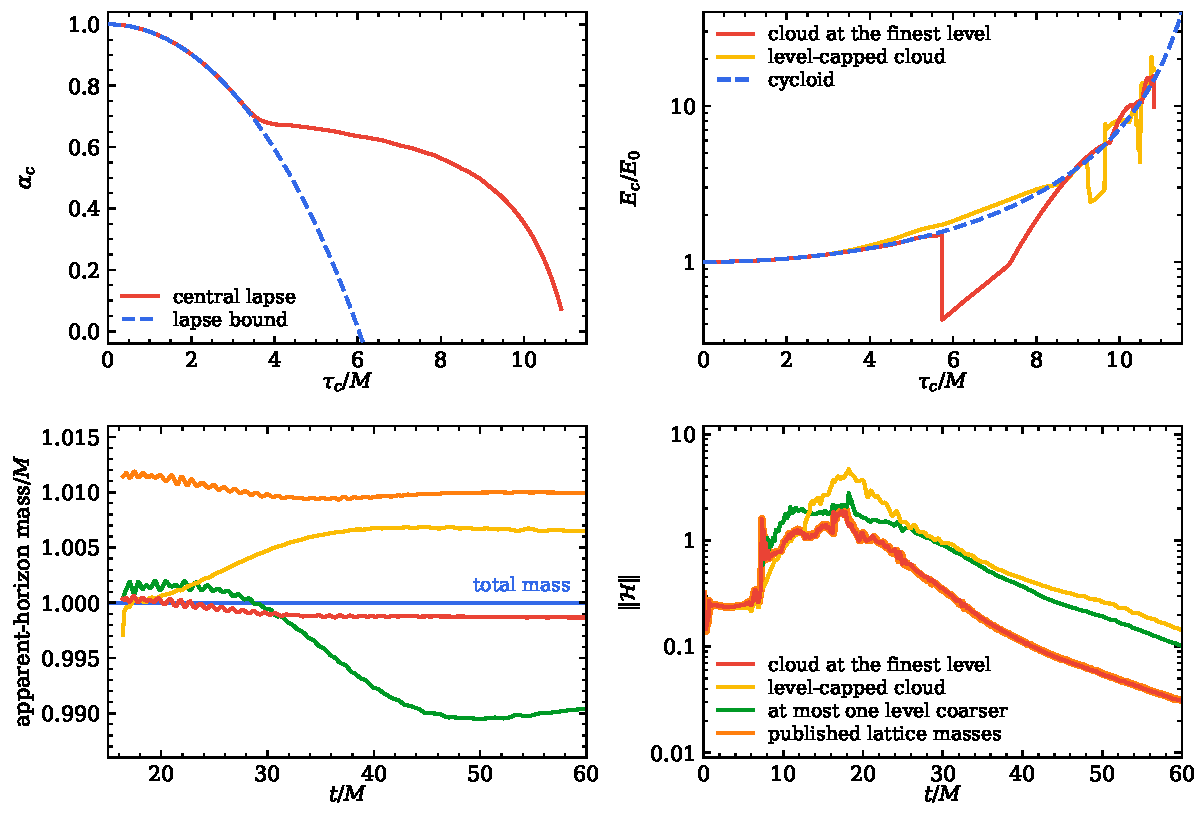
\includegraphics[width=\textwidth]{figures/fig_dust.pdf}
\caption{Gravitational collapse of a pressureless dust ball ($R_0 = 5\,M$, nearly $10^4$ macroparticles) to a black hole on an adaptive mesh. Top left: central lapse $\alpha_c$ versus central proper time $\tau_c$ (red) and the analytic lapse bound (blue dashed). Top right: central energy density $E_c/E_0$ and the cycloid (blue dashed) before central excision. Bottom: apparent-horizon mass with total mass $M$ (blue), and Hamiltonian constraint norm $\|\Ham\|$. Curves show finest-level clouds with surface-corrected (red) or published (orange, bottom) lattice masses, and level-capped clouds with unlimited (yellow) or one-level (green, bottom) coarsening.}
\label{fig:dust}
\end{figure*}

At $N \lesssim 10^4$, discrete lattice initialization must match the particle rest-mass sum to the continuum rest mass $M_0$ of the initial slice. With published lattice masses \cite{Wu:2026nrpic}, each site inside $\rbar_0$ carries rest mass $m_p = \rho_0 \psi(\bm{x}_p)^6 h^3$, the local proper rest-mass density times the cell volume. Those masses were first assumed to yield a black hole of mass $M$ here, as at $N \sim 10^6$ where surface count offsets vanish. At $N \lesssim 10^4$, however, the count of lattice sites inside a sphere differs from its volume in cells. On the lattice of Table~\ref{tab:setups} ($26$ cells across $2\rbar_0$), that count exceeds the cell volume and leaves $\sum_p m_p$ above $M_0$ (Table~\ref{tab:outcomes_dust}). Runs with published lattice masses kept the interior density exact, so $\alpha_c$ and $E_c$ still matched the surface-corrected collapse. Their apparent-horizon mass $M_{\rm AH}$, however, formed visibly above $M$ (Fig.~\ref{fig:dust}, bottom left, orange curve; Table~\ref{tab:outcomes_dust}). Radial profiles of the slice Misner--Sharp mass $M_{\rm MS}$ traced this excess to a mass shell leaving the boundary at $t = 0$ at light speed, outside which $M_{\rm MS}$ equaled $M$. The surface correction of Sec.~\ref{sec:numerical_methods} rescales $m_p$ in the outermost lattice layer of width $h$ so $\sum_p m_p = M_0$ with interior masses unchanged. With surface-corrected lattice masses, $M_{\rm AH}$ at formation matches $M$ to within the accuracy of the mass measure and drifts downward only slightly afterward (Fig.~\ref{fig:dust}, bottom left, red curve; Table~\ref{tab:outcomes_dust}).

Reliable horizon masses after collapse require checking the apparent-horizon finder on a vacuum black hole of known mass $M$ without matter or excision. In initial collapse tests, AthenaK's distributed pseudospectral flow finder \cite{Gundlach:1997us,2026ApJS..283...27S,Zhu:2024utz} returned horizon masses visibly below $M$. A first reading, that the flow iteration stopped too early, was ruled out on an evolved vacuum puncture of mass $M$ (Sec.~\ref{sec:evolving_black_hole}) when a much tighter stopping rule left the deficit unchanged. Across three cell spacings on that puncture, AthenaK's distributed finder reported masses well below $M$, with a deficit that is nonmonotonic in cell size (Fig.~\ref{fig:horizoncheck}, top panel, solid curves; Table~\ref{tab:outcomes}). On the same slices, we evaluated the slice Misner--Sharp mass $M_{\rm MS}$, the enclosed mass from slice geometry alone (Sec.~\ref{sec:numerical_methods}; Fig.~\ref{fig:horizoncheck}, open circles). Whereas $M_{\rm MS}$ fell short of $M$ on the coarsest mesh, it matched $M$ on the two finer meshes where the black hole is resolved (Table~\ref{tab:outcomes}). On those two resolved meshes, the evolved spacetime carried the mass $M$ and the deficit belonged to the finder. Inspection of the finder showed that it interpolates metric derivatives stored on active cells, whose ghost zones remain unfilled across block faces (Secs.~\ref{sec:numerical_methods} and \ref{sec:assembly}). Relative to $M_{\rm MS}$, the finder deficit is largest on the finest mesh, where blocks are narrowest and more block faces cut the origin-centered horizon. Direct differentiation of the ghost-filled Lagrange metric interpolant on the trial surface eliminates those block-face errors and restores spherical zero-expansion horizons. At the two finer cell sizes, the corrected apparent-horizon mass $M_{\rm AH}$ matches $M_{\rm MS}$ closely on saved slices and in a live run (Fig.~\ref{fig:horizoncheck}, dashed curve and diamonds; Table~\ref{tab:outcomes}).

\begin{figure}[t]
\centering
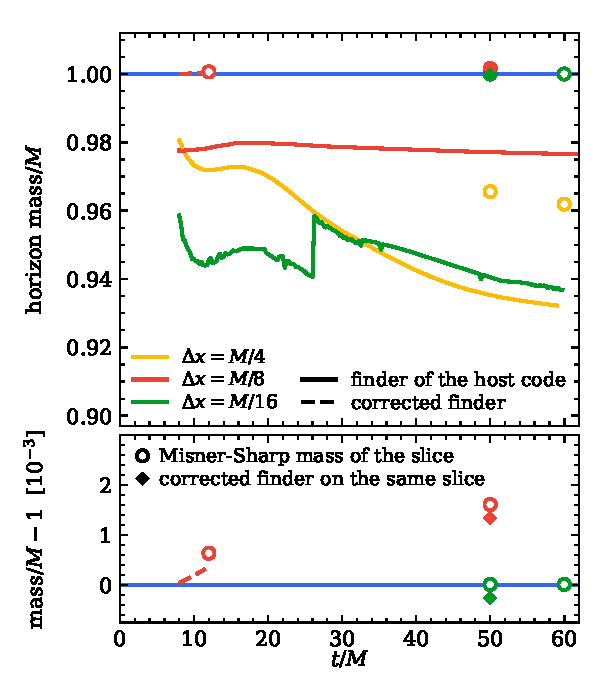
\includegraphics[width=\columnwidth]{figures/fig_horizon_check.pdf}
\caption{Apparent-horizon mass of a vacuum black hole of mass $M$ (blue) at three cell spacings (colors). Solid curves show the host code's finder, and the dashed curve differentiates the metric interpolant. Circles show the slice Misner--Sharp mass and diamonds the corrected finder on the same slices (enlarged below).}
\label{fig:horizoncheck}
\end{figure}

Level-capped deposition (Sec.~\ref{sec:deposition}) sets $\lcap$ from local particle density so sparse refined regions deposit onto virtual cloud cells of width near the initial particle spacing $h$. On the surface-corrected lattice, an unlimited cap removes the $\|\Ham\|$ jump when the center refines to $\Delta x = h/4$ (Fig.~\ref{fig:dust}, bottom right; Table~\ref{tab:outcomes_dust}). Although innermost particle radii stay identical across the runs, the central-density reading $E_c(\tau_c)$ then sits above the cycloid (Fig.~\ref{fig:dust}, top right, yellow curve). That excess arises because the contracting particle lattice beats against virtual cloud cells of nearly equal spacing $h$ at the center. Stored particles from the finest-level run reproduce these $E_c$ readings when redeposited onto width-$h$ clouds. Near the forming black hole, the unlimited cap raises $\|\Ham\|$ and drives $M_{\rm AH}$ above $M$ after excision. A one-level coarsening cap raises $E_c$ further (Table~\ref{tab:outcomes_dust}), elevates $\|\Ham\|$, and shifts $M_{\rm AH}$ to about one percent below $M$ (Fig.~\ref{fig:dust}, bottom panels, green curves).

Randomly sampled dust controls test finest-level against level-capped clouds at two refinement depths (Tables~\ref{tab:setups} and \ref{tab:outcomes_dust}). At full depth ($\Delta x = h/8$) under plain or compensated filtering, finest-level clouds follow sampling noise past the block limit before an apparent horizon forms. At that depth under either filter, level-capped clouds keep refinement bounded through black hole formation with $M_{\rm AH}$ within a few tenths of a percent of $M$. One refinement level shallower ($\Delta x = h/4$) with compensated filtering, both finest-level and level-capped runs complete on the same random sample. In that paired comparison without a lattice, level-capped clouds still raise $\|\Ham\|$ after black hole formation and shift $M_{\rm AH}$ lower by a few tenths of a percent (Table~\ref{tab:outcomes_dust}). That paired run refuted an initial explanation attributing the coarser-cloud disturbance to the lattice beat alone. Coarser clouds raise constraint residuals near a forming black hole and shift $M_{\rm AH}$ by a few tenths of a percent, more on a lattice, yet bound deep refinement on random samples. Finest-level clouds are more accurate where refinement stays bounded and are used for every production collapse run, while the level-capped runs serve as controls.

\subsection{Prolate collapse}\label{sec:prolate}

Cold prolate collapse from rest tests the coupled solver in three dimensions beyond spherical symmetry. Transverse infall focuses collisionless matter onto the symmetry axis into a caustic before any apparent horizon forms. Early axisymmetric simulations found rapidly growing curvature ahead of any apparent horizon \cite{Shapiro:1991zza}. Analytic examples showed that spatial slices of a black hole spacetime can miss trapped surfaces \cite{Wald:1991zz}. Three-dimensional particle runs later found resolution-dependent curvature peaks inside the spindle for this model \cite{Yoo:2016kzu}. Generalized-harmonic evolutions then followed collapse past the caustic to black hole formation \cite{East:2019bwu}. Particle-in-cell Z4c runs likewise formed an apparent horizon after the caustic \cite{Wu:2026nrpic}. A homogeneous spheroid of mass $M$ and eccentricity $e = 0.9$ starts from rest with $N = 10^4$ symmetric equal-mass macroparticles (Appendix~\ref{app:sampling}) on an adaptive mesh (Table~\ref{tab:setups}).

Radial infall contracts the spheroid into a thin spindle (Fig.~\ref{fig:prolate}, top row, at saved snapshots nearest the published times \cite{Wu:2026nrpic}). At $N = 10^4$ this spindle is an axial chain of separate condensations (Fig.~\ref{fig:prolate}, third panel). Equatorial reflection symmetry of the sample places two mirror-image maxima of the Kretschmann scalar $I$ (Sec.~\ref{sec:numerical_methods}) inside the matter on the axis, first near the ends \cite{Wu:2026nrpic}. Those maxima move inward in steps as peak $I$ jumps between condensations (Fig.~\ref{fig:prolate}, bottom left). Peak $I$ depends on cell spacing \cite{Wu:2026nrpic}, with an upward jump in Fig.~\ref{fig:prolate} when the finest mesh levels appear. With grid curvature finite throughout focusing, the run continues through the stage of largest curvature. An apparent horizon first forms at the time shown in Ref.~\cite{Wu:2026nrpic}, with spindle tips extending past its poles (Fig.~\ref{fig:prolate}). Lapse excision below $\aexc$ then removes all $10^4$ macroparticles as those tips fall into the black hole.

\begin{figure*}[t]
\centering
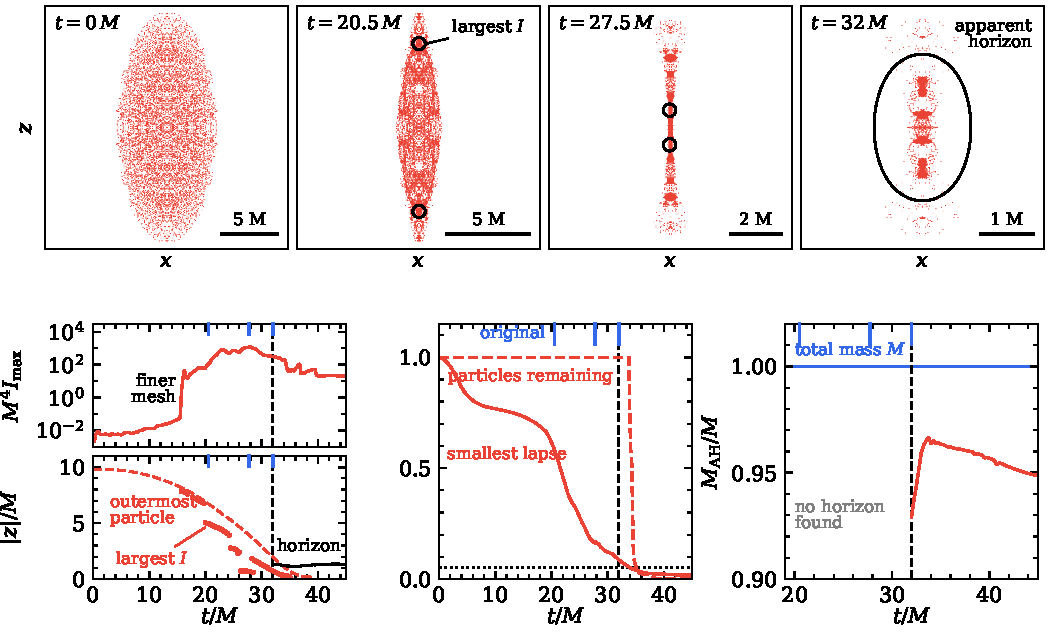
\includegraphics[width=\textwidth]{figures/fig_prolate.pdf}
\caption{The cold prolate spheroid ($e = 0.9$, $N = 10^4$) collapses into a segmented spindle whose two axial curvature maxima step inward before an apparent horizon forms. Top: $x$--$z$ macroparticles, maxima of the Kretschmann scalar $I$ (circles), and first apparent horizon (black). Bottom left: peak $I$, plus axial $|z|$ of that peak (red), outermost macroparticle (red dashed), and horizon (black). Bottom middle and right: smallest lapse with $\aexc$ (dotted) and surviving fraction (red dashed), and $M_{\rm AH}$ with $M$ (blue). Vertical dashed lines mark first horizon; blue ticks mark snapshot times \cite{Wu:2026nrpic}.}
\label{fig:prolate}
\end{figure*}

The apparent-horizon mass $M_{\rm AH}$ (Sec.~\ref{sec:numerical_methods}) peaks about five percent below $M$ after polar infall (Fig.~\ref{fig:prolate}, bottom right; Table~\ref{tab:outcomes_prolate}). That apparent-horizon mass continues to fall at the end of the run. Reference~\cite{Wu:2026nrpic} states no apparent-horizon mass for this test. The slice Misner--Sharp mass $M_{\rm MS}$ (Sec.~\ref{sec:numerical_methods}) on the final slice agrees with the finder at the apparent horizon within its angular spread (Table~\ref{tab:outcomes_prolate}). The same profile $M_{\rm MS}$ recovers the total mass $M$ at large radius. The remaining five to eight percent of $M$ after lapse excision reside in gravitational fields outside the black hole (Table~\ref{tab:outcomes_prolate}). Outside the black hole, $M_{\rm MS}(R) - M_{\rm AH}$ sums radiated gravitational-wave energy and geometric mass from constraint violations without separating them. The Hamiltonian constraint norm $\|\Ham\|$ peaks at largest curvature about three times above its lattice dust peak (Sec.~\ref{sec:dust}; Table~\ref{tab:outcomes_prolate}). A spherical control with a random sample and the same filter loses only a few tenths of a percent of $M$, so random sampling alone does not explain this deficit. How the deficit of the prolate collapse splits between particle number and cell size at its caustic stage is not determined. Dynamic refinement (Sec.~\ref{sec:amr}) with halved finest cells exceeds the block memory of one graphics card, which sets our finest grid.

On the prolate sample at $\Delta x = M/32$, four binomial passes with compensation (Sec.~\ref{sec:deposition}) remove only the early noise-driven refinement. Curvature along the collapsing spindle itself still drives the block count past the memory limit before an apparent horizon forms. The production run stays bounded because its refinement depth is limited by one level ($\Delta x = M/16$) alongside that compensated filter (Table~\ref{tab:setups}).

\subsection{Relativistic clusters}\label{sec:clusters}

Warm collisionless star clusters in equilibrium balance collective gravity through velocity dispersion. Their evolution tests phase-space conservation alongside general-relativistic radial stability \cite{1968ApJ...154..251I,1980ApJ...238.1101I,1985ApJ...298...34S,1985ApJ...298...58S}. As in Shapiro and Teukolsky \cite{1985ApJ...298...34S,1985ApJ...298...58S} and Ref.~\cite{Wu:2026nrpic}, static, spherically symmetric, isotropic monoenergetic (single-energy) clusters populate one Killing energy $\Egeo = \alpha W = \alpha_{\rm s}$. Here $\alpha_{\rm s}$ is the lapse at the cluster surface, where particle speed vanishes ($W = 1$). Radial integration of the Einstein-Vlasov equilibrium relations---the structure equations---yields a one-parameter sequence labeled by $y_c \in (0, 1)$, with gravitational binding energy $E_b$,
\begin{equation}\label{eq:cluster_sequence}
y_c = \left(\frac{\alpha_{c,\rm eq}}{\alpha_{\rm s}}\right)^2, \qquad
E_b = M_0 - M.
\end{equation}
In this sequence, $\alpha_{c,\rm eq}$ is the equilibrium central lapse, $z_c = \alpha_{c,\rm eq}^{-1} - 1$ is the central redshift, $M_0$ is total rest mass, and $M$ is ADM mass \cite{1985ApJ...298...34S,Andreasson:2011ng}. From diffuse, nearly Newtonian clusters ($y_c \to 1$, low $z_c$) to compact, relativistic cores (smaller $y_c$, high $z_c$), $E_b/M_0$ rises to one maximum along the sequence. At still smaller $y_c$, $E_b$ decreases and turns negative ($M > M_0$). Like the turning point of fluid stars \cite{Chandrasekhar:1964zz,Friedman:1988er}, that binding-energy maximum separates stable clusters at larger $y_c$ from unstable clusters at smaller $y_c$ \cite{1980ApJ...238.1101I,1985ApJ...298...58S,Wu:2026nrpic}. Perturbed clusters on the high-$y_c$ branch hold together, whereas clusters past the maximum collapse or expand. Each unit-mass cluster draws up to $10^4$ equal-mass macroparticles with zero net momentum (Sec.~\ref{sec:numerical_methods}). Static meshes evolve the two loosest models and adaptive meshes evolve the kicked compact ones, with all meshes and particle numbers in Table~\ref{tab:setups}.

Multi-pass grid filtering suppresses discrete source fluctuations at $N = 10^4$, yet uncompensated smoothing biases self-gravitating equilibria outward. An unperturbed cluster on the stable branch ($y_c = 0.819$) was expected to stay near equilibrium with minor oscillations, as for the kicked model in Ref.~\cite{Wu:2026nrpic}. With four plain binomial passes, the cluster instead expanded by a visible fraction of its radius and dropped in central density before rebounding. Over that bounce, $\alpha_c$ rose well above $\alpha_{c,\rm eq}$ (Fig.~\ref{fig:filter}, left panel, solid curves; Table~\ref{tab:outcomes_clusters}). A first reading, that discrete sampling noise drove this excursion, was ruled out when three independent $10^4$-particle samples traced the identical bounce up to a tiny ripple (Fig.~\ref{fig:filter}, left panel). Sweeps across zero, two, and four plain passes on one sample showed that the initial lapse rise grows systematically with pass count $n_{\rm f}$ (Fig.~\ref{fig:filter}, middle panel). Each plain binomial pass widens every cloud's second moment, which acts as a gravitational softening over the filter scale \cite{2008gady.book.....B} (Sec.~\ref{sec:deposition}). Plain passes also lower the proper-volume integral of $E$ slightly across nonuniform $\sqrt{\gamma}$. Because particle velocities match the unsoftened equilibrium, that shallower smoothed potential lets the cluster expand and recontract. The compensation pass of Sec.~\ref{sec:deposition} \cite{1991ppcs.book.....B} cancels that second-moment softening and preserves the proper-volume energy integral. It removes the bounce across two and four passes and leaves $\alpha_c(t)$ insensitive to $n_{\rm f}$ (Fig.~\ref{fig:filter}, dashed curves). Unfiltered evolution ($n_{\rm f} = 0$) also avoids the bounce, yet leaves $\|\Ham\|$ much higher (Table~\ref{tab:outcomes_clusters}) and causes $\alpha_c$ to wander downward later (Fig.~\ref{fig:filter}, middle panel). All cluster runs below therefore combine four binomial passes with compensation.

\begin{figure*}[t]
\centering
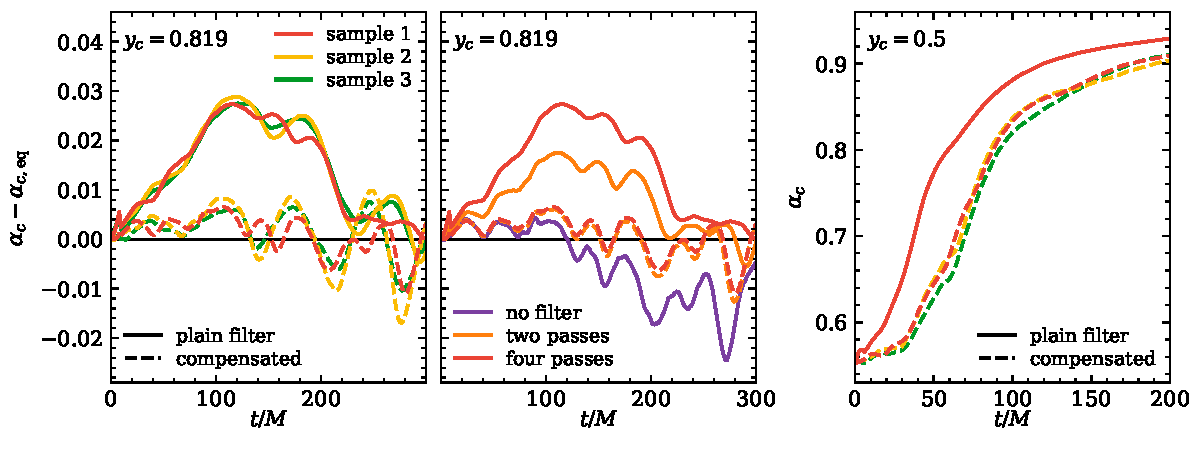
\includegraphics[width=\textwidth]{figures/fig_filter.pdf}
\caption{Source filtering and radial motion of monoenergetic clusters with $N = 10^4$ macroparticles. Left: central-lapse offset $\alpha_c - \alpha_{c,\rm eq}$ from equilibrium (black line) for the stable model $y_c = 0.819$ across three samples (colors), comparing four plain binomial passes (solid) with compensated filtering (dashed). Middle: one sample with zero, two, and four filter passes (colors), plain (solid) and compensated (dashed). Right: central lapse $\alpha_c$ of the unperturbed unstable model $y_c = 0.5$, encoded as on the left.}
\label{fig:filter}
\end{figure*}

Dynamically stable clusters on the high-$y_c$ side of the binding-energy maximum are expected to remain bound and oscillate stably under small radial perturbations. As in Ref.~\cite{Wu:2026nrpic}, we apply a one-percent inward velocity kick to the stable models $y_c = 0.900$ and $y_c = 0.819$ at $N = 10^4$ (Fig.~\ref{fig:clusters}, first two columns). Over several crossing times, both clusters retain every macroparticle and stay centered near the origin, as in Ref.~\cite{Wu:2026nrpic}. Rest-mass radii stay within a narrow band for $y_c = 0.900$ and undergo bounded radial swings in the inner shells of $y_c = 0.819$ (Fig.~\ref{fig:clusters}, top left). Because its potential is shallower, the looser model $y_c = 0.900$ shows much smaller variations in $\alpha_c$ (Table~\ref{tab:outcomes_clusters}) and mean Lorentz factor than $y_c = 0.819$.

\begin{figure*}[t]
\centering
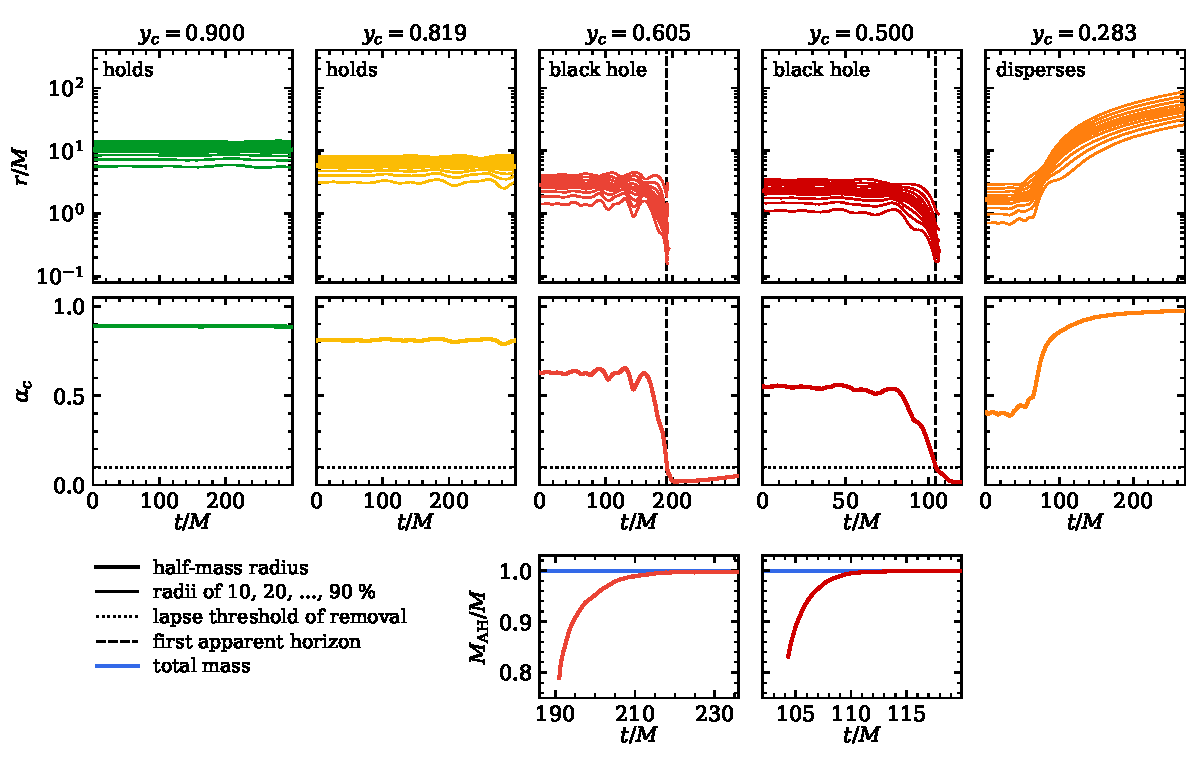
\includegraphics[width=\textwidth]{figures/fig_clusters.pdf}
\caption{Five monoenergetic clusters ($N = 10^4$) with an inward velocity kick, ordered from least compact (left) to most compact (right). Models $y_c = 0.900$ and $0.819$ hold, $0.605$ and $0.500$ form black holes, and the unbound model $0.283$ disperses. Top: coordinate radii enclosing tenths of remaining rest mass (half-mass thicker) while at least half remains. Middle: central lapse $\alpha_c$ with excision threshold $\aexc$ (dotted) and first apparent horizon (dashed, also top). Bottom: apparent-horizon mass $M_{\rm AH}$ and total mass $M$ (blue).}
\label{fig:clusters}
\end{figure*}

Closer inspection of the stable model $y_c = 0.819$ reveals a coherent radial oscillation of its core that grows before saturating at late times. With filter softening removed, an unperturbed equilibrium was expected to hold a steady central lapse $\alpha_c = \alpha_{c,\rm eq}$. Instead, $\alpha_c$ oscillates at a period close to the radial period of a particle in the core (Fig.~\ref{fig:oscillation}, top panel; Table~\ref{tab:outcomes_clusters}), while the outer shells stay within a few percent of their initial radii over the first three hundred $M$ and move more afterward. Because a nearly uniform core creates an almost harmonic potential with a shared radial period, collective core motion resists phase mixing \cite{2008gady.book.....B}. Over the first several periods the swing grows steadily, so a long continuation tested unbounded instability against saturation. In that extended run, growth halts after several cycles and the swing stays bounded at a small fraction of $\alpha_{c,\rm eq}$ with all $10^4$ particles retained (Fig.~\ref{fig:oscillation}, top panel). A first reading, that intermediate-wavenumber sampling noise passed by the compensated filter excited this mode, was ruled out by three stratified samples (Fig.~\ref{fig:oscillation}, top panel) and a Monte Carlo sample. All samples share the same period, phase, and growth. Inward-kicked runs at $N = 10^3$ and $10^4$ likewise show matching early swings without $N^{-1/2}$ amplification (Fig.~\ref{fig:oscillation}, bottom left; Table~\ref{tab:outcomes_clusters}).

Further controls on the first sample tested whether time-stepping lag, constraint handling, cloud width, or cell spacing drives this core oscillation (Fig.~\ref{fig:oscillation}, bottom middle and right; Table~\ref{tab:setups}). Frozen sources across $\Delta t$ could lag particle motion, yet a halved step $\Delta t/2$ leaves $\alpha_c(t)$ unchanged. Feedback from constraint damping or advected constraint residuals was tested across raised and zero $\kappa_1$ and with parabolic relaxation of the Hamiltonian constraint (Sec.~\ref{sec:spacetime}). Although those settings alter $\|\Ham\|$ substantially, all three reproduce $\alpha_c(t)$ to a tiny fraction of the swing (Fig.~\ref{fig:oscillation}, bottom right; Table~\ref{tab:outcomes_clusters}). An extended compensation weight $c$ that also cancels cloud width trims the slow excursion slightly while leaving the oscillation intact (Fig.~\ref{fig:oscillation}, bottom middle; Table~\ref{tab:outcomes_clusters}). A control with halved cell spacing over the cluster (Table~\ref{tab:setups}) leaves the first $\alpha_c$ maximum unchanged, gives an equal or slightly larger growth rate, and drifts further in mean lapse. That control refutes a second-order cell-size origin for the oscillation. In the sequence figure of Ref.~\cite{Wu:2026nrpic}, the full-range lapse axis is too coarse to resolve a swing of $0.01$ in $y_c = 0.819$. By contrast, the narrower-axis figure for the perturbed near-critical cluster in Ref.~\cite{Wu:2026nrpic} at $N = 10^6$ displays the same growth, saturation, and decay at the core period. What sets the small common initial offset from which the unperturbed oscillation starts here is not determined.

\begin{figure*}[t]
\centering
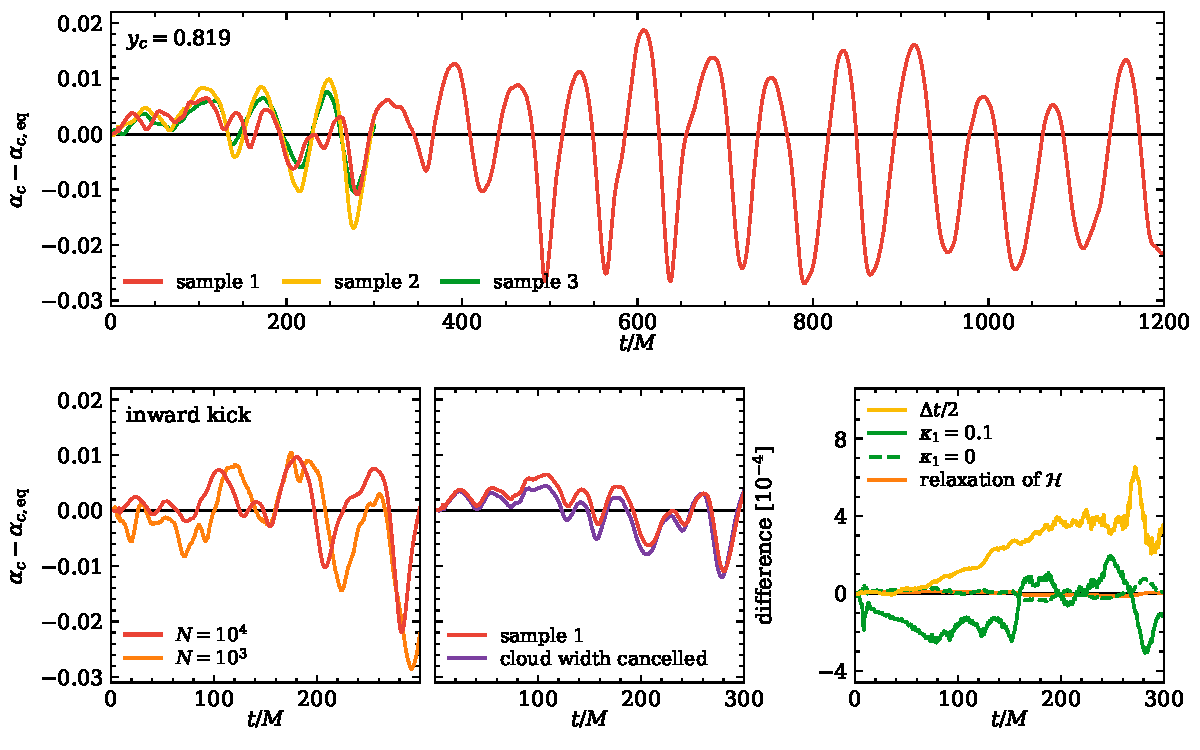
\includegraphics[width=\textwidth]{figures/fig_oscillation.pdf}
\caption{Core oscillation of the stable cluster $y_c = 0.819$ in central-lapse offset $\alpha_c - \alpha_{c,\rm eq}$ from equilibrium (black lines). Top: three unperturbed samples at $N = 10^4$ (colors), with sample 1 continued to saturation. Bottom left: inward-kicked runs at $N = 10^4$ and $10^3$. Bottom middle: sample 1 against compensation that also cancels cloud width. Bottom right: differences from sample 1 for $\Delta t/2$, raised and zero (dashed) constraint damping $\kappa_1$, and relaxation of the Hamiltonian constraint.}
\label{fig:oscillation}
\end{figure*}

Smaller counts $N$ at fixed mass $M$ amplify force fluctuations as $N^{-1/2}$ and hasten collisional heating. Stratified and Monte Carlo runs of $y_c = 0.819$ across $N = 10^4$, $10^3$, and $10^2$ locate where graininess overtakes collective dynamics (Table~\ref{tab:setups}). At $N = 10^3$, the cluster holds together and follows the $N = 10^4$ oscillation across several periods (Fig.~\ref{fig:oscillation}, bottom left). Later cycles at $N = 10^3$ develop deeper lapse minima and a slow downward drift. At $N = 10^2$, discrete fluctuations overtake the cluster within one period. Net momentum wanders, mean kinetic energy more than doubles, and $\alpha_c$ plunges steadily as equilibrium breaks down (Table~\ref{tab:outcomes_clusters}). Both the $N = 10^4$ and $10^3$ clusters hold across the comparison run, whereas the $N = 10^2$ cluster loses equilibrium.

Past the binding-energy maximum the clusters are unstable \cite{1980ApJ...238.1101I,1985ApJ...298...58S}. Reference~\cite{Wu:2026nrpic} finds collapse under an inward kick for the bound models past that maximum ($E_b > 0$) and dispersal for the unbound model ($E_b < 0$). With the one-percent inward kick on adaptive meshes, both bound unstable models $y_c = 0.605$ and $y_c = 0.500$ collapse to black holes (Fig.~\ref{fig:clusters}, third and fourth columns). Once infall accelerates, mass shells contract together, $\alpha_c$ plunges toward zero, and an apparent horizon forms. As outer shells accrete, $M_{\rm AH}$ rises rapidly to $M$ while lapse excision removes almost every macroparticle (Fig.~\ref{fig:clusters}, bottom panels; Table~\ref{tab:outcomes_clusters}). Black hole formation and full mass capture agree with Ref.~\cite{Wu:2026nrpic}, alongside two documented differences. First, apparent horizons form later here for both $y_c = 0.605$ and $y_c = 0.500$ than in Ref.~\cite{Wu:2026nrpic} (Table~\ref{tab:outcomes_clusters}). Reference~\cite{Wu:2026nrpic} notes that these collapse times could depend on $N$ and initial sampling noise. In $y_c = 0.605$, a growing core oscillation also precedes collapse (Fig.~\ref{fig:clusters}, third column), whereas the published lapse falls smoothly. The cause of these later collapse times is not determined. Second, after horizon formation $\alpha_c$ settles closer to zero here than in Ref.~\cite{Wu:2026nrpic}. This difference concerns the coordinates at the center, and its origin was not looked into. For the unbound cluster $y_c = 0.283$ ($E_b < 0$), $\alpha_c$ dips briefly after the kick before rebounding into free dispersal (Fig.~\ref{fig:clusters}, rightmost column). Its central lapse approaches unity and mass shells expand at constant asymptotic speeds with every macroparticle kept. This free dispersal agrees with Ref.~\cite{Wu:2026nrpic}, whereas early spherical runs \cite{1985ApJ...298...58S} reported black hole formation.

Without a kick, an unstable cluster past the binding-energy maximum can expand dynamically toward the stable branch of equal mass, a nonlinear transition termed migration \cite{Font:2001ew,Wu:2026nrpic}. Because the same model $y_c = 0.5$ expands when unperturbed in Ref.~\cite{Wu:2026nrpic} whereas kicked $y_c = 0.500$ collapses, we first asked whether plain-filter softening alone selected expansion over collapse. Paired runs of unperturbed $y_c = 0.5$ with plain and compensated four-pass filtering tested that hypothesis directly (Fig.~\ref{fig:filter}, right panel). Plain filtering advances the expansion noticeably, yet three compensated samples still expand outward on a common schedule (Fig.~\ref{fig:filter}, right panel). Plain filtering therefore hastens an already outward transition. In the full run on a static mesh with compensation, the unperturbed cluster $y_c = 0.5$ expands strongly and then recontracts deeply (Fig.~\ref{fig:migration}; Table~\ref{tab:setups}). After that rebound, the cluster settles into a damped oscillation about a more extended state to the end of the run. The sequence of states and the first two maxima and minima of $\alpha_c$ agree with the migration curve of Ref.~\cite{Wu:2026nrpic} (Table~\ref{tab:outcomes_migration}). After the first maximum, every extremum of $\alpha_c$ arrives earlier here than in Ref.~\cite{Wu:2026nrpic}, and the later swings are smaller. Once the cluster expands, most matter lies outside the finest central box of this static mesh on coarser cells, whereas Ref.~\cite{Wu:2026nrpic} refines adaptively (Table~\ref{tab:setups}). Whether the coarser outer mesh, lower $N$, or filter compensation causes those timing and amplitude differences is not determined. Over the run, four macroparticles leave the domain and none is removed by lapse excision (Table~\ref{tab:outcomes_migration}).

\begin{figure}[t]
\centering
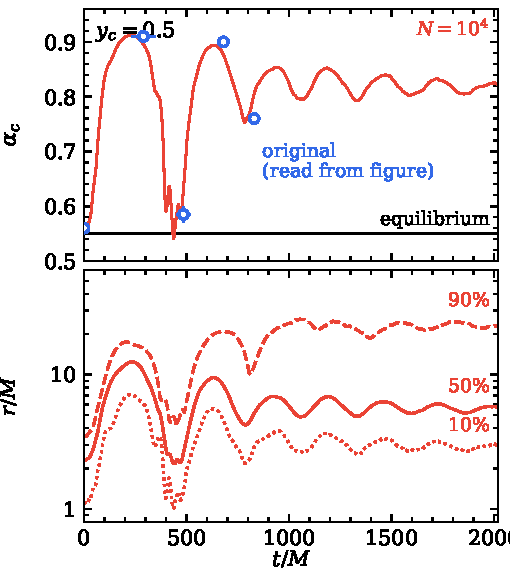
\includegraphics[width=\columnwidth]{figures/fig_migration.pdf}
\caption{The unperturbed cluster $y_c = 0.5$ expands, recontracts deeply, and oscillates with decreasing swing about a more extended state. Top: central lapse $\alpha_c$, equilibrium (black), and extrema from Ref.~\cite{Wu:2026nrpic} (circles; bars: read ranges). Bottom: radii enclosing the labeled rest-mass fractions.}
\label{fig:migration}
\end{figure}

Near the binding-energy maximum, Ref.~\cite{Wu:2026nrpic} applies a ten-percent initial density perturbation to $y_c = 0.756$ at $N = 10^6$. It reports reconfiguration into a persistent core--halo structure with all macroparticles retained, damped early lapse oscillations, and a slow fall of $\alpha_c$. Its text states the amplitude of the perturbation and leaves its sign and the initial-metric construction open. Over the shorter runs here, the comparison is limited to $\alpha_c$ and the enclosed rest-mass radii shown in Fig.~\ref{fig:nearcritical}. Here homologous radial scaling changes the density by ten percent of either sign while $\psi$ solves $\Ham = 0$ for the perturbed matter (Appendix~\ref{app:sampling}). Under ten-percent compression, the cluster contracts and collapses to a black hole with every macroparticle removed by lapse excision (Fig.~\ref{fig:nearcritical}; Tables~\ref{tab:setups} and \ref{tab:outcomes_migration}). The final apparent-horizon mass equals the ADM mass of the compressed initial data. A control run with the compressed particles on the unperturbed equilibrium metric contracts in the same way. Under ten-percent expansion, the cluster oscillates and keeps every macroparticle (Fig.~\ref{fig:nearcritical}). Its oscillation runs about a higher central lapse and with a slower rhythm than the published $\alpha_c$ curve of Ref.~\cite{Wu:2026nrpic}. The unperturbed model $y_c = 0.756$ oscillates about its equilibrium at the core period with a swing that grows and then stops growing (Fig.~\ref{fig:nearcritical}). Its mean lapse falls slowly below the equilibrium value over the run, as in the published $\alpha_c$ curve. That $\alpha_c$ evolution matches the core oscillation of the stable model in Fig.~\ref{fig:oscillation} and, apart from a time shift, resembles the published $\alpha_c$ curve in Ref.~\cite{Wu:2026nrpic} most closely (Table~\ref{tab:outcomes_migration}). As an interpretation, the oscillation in the published figure may be this intrinsic core oscillation, while which perturbation Ref.~\cite{Wu:2026nrpic} applied cannot be decided from its text.

\begin{figure}[t]
\centering
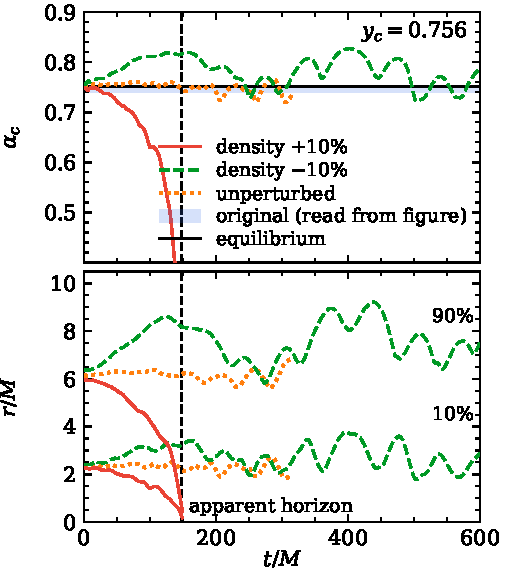
\includegraphics[width=\columnwidth]{figures/fig_nearcritical.pdf}
\caption{The near-critical cluster $y_c = 0.756$ collapses to a black hole when compressed, oscillates when expanded, and shows the core oscillation when unperturbed. Top: central lapse $\alpha_c$, first apparent horizon (dashed), and extrema from Ref.~\cite{Wu:2026nrpic} (circles). Bottom: radii enclosing the labeled rest-mass fractions.}
\label{fig:nearcritical}
\end{figure}
